%----------------------------------------------------------------------------
\chapter{GraphWalker}\label{sect:GraphWalker implementation of Garage Gate model}

%----------------------------------------------------------------------------
\section{GraphWalker}
%----------------------------------------------------------------------------

\section{GraphWalker implementation in Eclipse}

 We can connect more models with the \textit{SHARED:someName} keyword in a vertex. Consequently I have created a yEd graph model for test scenarios for the garage gate state machine (see \figref{Garage Statemachine}), and a graph model for the lamp, which called from the previous graph.

\begin{figure}[!ht]
	\centering
	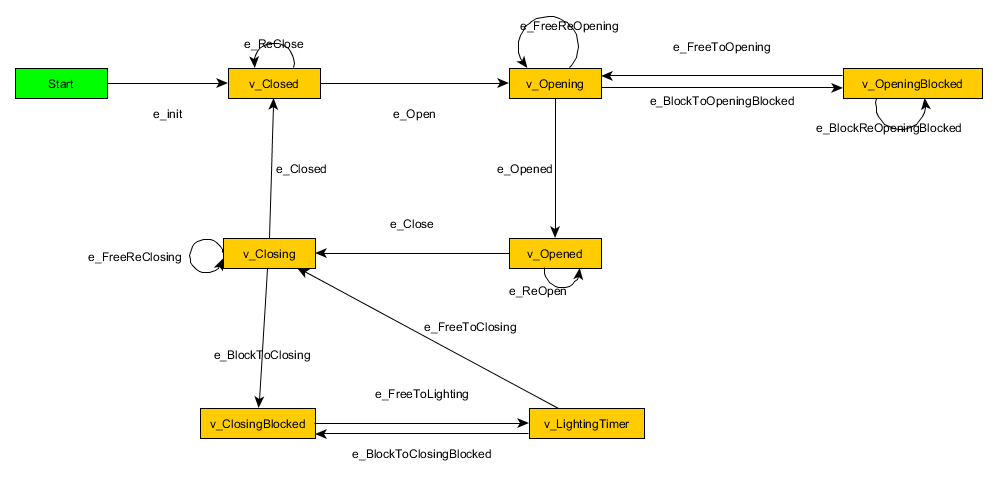
\includegraphics[width=150mm, keepaspectratio]{figures/GateModel.png}
	\caption{Garage gate model with yEd}
	\label{fig:GateModel}
\end{figure}

\begin{figure}[!ht]
	\centering
	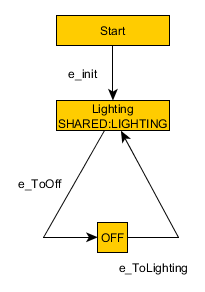
\includegraphics[width=50mm, keepaspectratio]{figures/LightingModel.png}
	\caption{Lamp0 model with yEd}
	\label{fig:LampModel}
\end{figure}


Generated test with option: @GraphWalker(start = "e\_init", value = "random(vertex\_coverage(100))"), and the result was:
[INFO] Result :
[INFO] 
[INFO] {
	"totalFailedNumberOfModels": 0,
	"totalNotExecutedNumberOfModels": 0,
	"totalNumberOfUnvisitedVertices": 0,
	"verticesNotVisited": [],
	"totalNumberOfModels": 2,
	"totalCompletedNumberOfModels": 2,
	"totalNumberOfVisitedEdges": 14,
	"totalIncompleteNumberOfModels": 0,
	"edgesNotVisited": [
	{
		"modelName": "GateModel",
		"edgeId": "e0",
		"edgeName": "e\_init"
	},
	{
		"modelName": "GateModel",
		"edgeId": "e3",
		"edgeName": "e\_Close"
	},
	{
		"modelName": "GateModel",
		"edgeId": "e10",
		"edgeName": "e\_FreeToOpening"
	},
	{
		"modelName": "GateModel",
		"edgeId": "e13",
		"edgeName": "e\_BlockReOpeningBlocked"
	}
	],
	"vertexCoverage": 100,
	"totalNumberOfEdges": 18,
	"totalNumberOfVisitedVertices": 9,
	"edgeCoverage": 77,
	"totalNumberOfVertices": 9,
	"totalNumberOfUnvisitedEdges": 4
}

%TODO implement PyModel stuff
\section{PyModel implementation}